\section{Evaluation}
\label{sec:eval}

\begin{figure*}
\centering
    \subfigure[LDA]{
        \label{fig:exp_lda}
        %\includegraphics[width=0.3\linewidth]{figures/fig_10B17_case1}
        \includegraphics[width=0.3\linewidth]{figs/exp_lda.eps}
    }
    \subfigure[GMM]{
        \label{fig:exp_gmm}
        %\includegraphics[width=0.3\linewidth]{figures/fig_15B31_case2}
        \includegraphics[width=0.3\linewidth]{figs/exp_slda.eps}
    }
    \subfigure[TwoCoins]{
        \label{fig:exp_twocoins}
        %\includegraphics[width=0.3\linewidth]{figures/fig_15B31_case2}
        \includegraphics[width=0.3\linewidth]{figs/exp_slda.eps}
    }
    \subfigure[DCMLDA]{
        \label{fig:exp_dcmlda}
        %\includegraphics[width=0.3\linewidth]{figures/fig_48B48_case6}
        \includegraphics[width=0.3\linewidth]{figs/exp_dcmlda.eps}
    }
	\caption{Running Time}
    \label{fig:exp_comparison}
\end{figure*}

In this section, we first present performance evaluation of InferSpark,
by constructing and carrying out statistic inference on four Bayesian
network models:
Latent Dirichlet Allocation (LDA), Dirichlet Compound Multinomial LDA
(DCMLDA)~\cite{Doyle2009}, Gaussian Mixture Model (GMM), and simple two-coin
model (TC). LDA is a standard model in topic modeling,
which takes in a collection of documents
and infers the topics of the documents.
DCMLDA is a cutomized topic model that accounts for burstiness in documents.
<<<<<<< HEAD
\KZ{Say a bit more about DCMLDA? GMM is ...}
All models can be implemented in InferSpark with fewer than 9 lines of code.
=======
\KZ{Describe a bit more about GMM is ...}
All models can be implemented in InferSpark with fewer than 9 lines of code. 
>>>>>>> 4fbb2be1662705a7274f07f5c9a919233d33b804
%(see \figref{fig:intro_lda_def} and Appendix \ref{models}).
For comparison, we include MLlib in our study whenever applicable.
MLlib includes LDA as a standard model.
However, it does not have support for DCMLDA, GMM \footnote{GMM can be solved
by EM algorithm on MLlib, but no statistical inference is possible.}
and TC. There are other probabilistic programming frameworks apart from
Infer.NET (see Section \ref{sec:related}).
<<<<<<< HEAD
All of them are unable to scale-out onto multiple machines yet.
Infer.NET so far is the most predominant one with the best performance, so we also include it in our study whenever applicable.
=======
All of them are unable to scale-out onto multiple machines yet.  
Infer.NET so far is the most predominant one with the best performance, 
so we include it in our study whenever applicable.
>>>>>>> 4fbb2be1662705a7274f07f5c9a919233d33b804

All the experiments are done on a 30-node Linux cluster, where each node
has a 2.6GHz quad-core, 32GB memory, and 700GB hard disk.
Spark 1.4.1 with scala 2.11.6 is installed on all nodes.
The default cluster size for InferSpark and MLlib is 24 data nodes
and 1 master node.  Infer.NET can only use one such node.
<<<<<<< HEAD
\KZ{The data sets for each of the four models are listed in Table \ref{data}.}
The Wikidataset is the Wikipedia dump~\cite{wikidump}.
=======
The data sets for each of the four models are listed in Table \ref{data}.
The Wikidataset is the Wikipedia dump~\cite{}. 
>>>>>>> 4fbb2be1662705a7274f07f5c9a919233d33b804
%Amazon is a dataset of Amazon reviews used in \cite{Jo2011}.
We run 50 iterations and do checkpointing every 10 iterations
for each model on each dataset.

Then we show how the partitioning strategy and the optimization on GraphX
improve the scalability of InferSpark. In these experiments,
no checkpoints are taken.

\begin{table}\scriptsize
\caption{Datasets}
\label{data}
\small
\begin{tabular}{ccc}
     \begin{tabular}{|c|c|c|}     \hline
        {Wiki} & words & topics \\\hline\hline
         1\% & 2,596,155  & 96 \\         \hline
         2\% & 5,192,310  & 96 \\         \hline
         \multicolumn{3}{c}{LDA} \\
     \end{tabular}
          &
     \begin{tabular}{|c|c|c|}     \hline
        {Wiki} & words & topics \\\hline\hline
         1\% & 2,596,155  & 10 \\         \hline
         2\% & 5,192,310  & 10 \\         \hline
         \multicolumn{3}{c}{DCMLDA} \\
     \end{tabular}
     \\\\
%     \begin{tabular}{|c|c|c|}     \hline
%        {Amazon} & words & topics \\\hline\hline
%         6\% & 349,569 & 96 \\\hline
%         10\% & 607,430  & 96 \\         \hline
%         \multicolumn{3}{c}{SLDA} \\
%     \end{tabular}
     \begin{tabular}{|c|c|c|}     \hline
        {Wiki} & words & topics \\\hline\hline
         0.5\% & 1,324,816 & 10 \\\hline
         1\% & 2,596,155  & 10 \\         \hline
         \multicolumn{3}{c}{GMM} \\
     \end{tabular}
&
     \begin{tabular}{|c|c|c|}     \hline
        {Wiki} & words & topics \\\hline\hline
         0.5\% & 1,324,816 & 10 \\\hline
         1\% & 2,596,155  & 10 \\         \hline
         \multicolumn{3}{c}{TC} \\
     \end{tabular}
\end{tabular}
\end{table}

\subsection{Overall Performance}
\KZ{Revise the following according to our actual results.}
\figref{fig:exp_comparison} shows the time of running LDA, DCMLDA, GMM and
TC on InferSpark, Infer.NET, and MLlib.
Infer.NET cannot finish the inference tasks on all four models within a day.
MLlib supports only LDA, and is more efficient than InferSpark in that case.
However, we remark that MLlib uses the EM algorithm which only
<<<<<<< HEAD
calculates Maximum A Posterior instead of the full posterior and is specific to LDA.
In contrast, InferSpark aims to provide a handy programming platform for statistician and domain users to build and test various customized models based on big data.
It would not be possible to be done by any current probabilistic frameworks nor with Spark/GraphX directly unless huge programming effort is devoted.
MLlib versus InferSpark
is similar to C++ programs versus DBMS: highly optimized C++ programs are more efficient,
=======
calculates maximum a posterior instead of the full posterior and 
is specific to LDA.
In contrast, InferSpark aims to provide a handy programming platform 
for statistician and domain users to build and test various customized 
models based on big data.
%It would not be possible to be done by any current probabilistic frameworks nor with Spark/GraphX directly unless huge programming effort is devoted.  
MLlib versus InferSpark is analogous to C++ programs versus DBMS: 
highly optimized C++ programs are more efficient, 
>>>>>>> 4fbb2be1662705a7274f07f5c9a919233d33b804
but DBMS achieves good performance with lower development time.
From now on, we focus on evaluating the performance of InferSpark.

Table \ref{breakdown} shows the time breakdown of InferSpark.
The inference process executed by GraphX, as expected,
dominates the running time.
The MPG construction step executed by Spark, can finish within two minutes.
The Bayesian network construction and code generation can be done in seconds.

\begin{table*}
\caption{Time Breakdown (in seconds and \%)}
\label{breakdown}
\centering
\small
\begin{tabular}{|l||*{8}{r|}r|}
\hline
Model & \multicolumn{2}{c|}{B.N. Construction} & \multicolumn{2}{c|}{Code Generation}	& \multicolumn{4}{c|}{Execution} & Total \\\cline{6-9}
  & \multicolumn{2}{c|}{ } & \multicolumn{2}{c|}{ }	& \multicolumn{2}{c|}{MPG Construction} & \multicolumn{2}{c|}{Inference} &	 \\ \hline \hline
LDA 541644 words	& 21.911	& 1.34\%	& 11.15 &	0.68\%	& 38.147	& 2.33\% &	1566.692 & 95.65\%	& 1637.9 \\ \hline
LDA 1324816 words &	21.911 & 0.70\% & 12.25	& 0.39\% & 79.4 & 2.55\%	& 3002.1 & 96.36\% &	3115.661 \\ \hline
DCMLDA 1324816 words & 22.658 & 0.65\%	& 10.52 & 0.30\% &	20.923	& 0.60\% & 3448.699	& 98.46\% &	3502.8 \\ \hline
DCMLDA 2596155 words & 22.658 & 0.28\% & 11.55 & 0.14\%	& 39.549 & 0.48\%	& 8153.969 & 99.10\%	& 8227.726 \\ \hline
GMM XXX nodes & 22.658 & 0.28\% & 11.55 & 0.14\%	& 39.549 & 0.48\%	& 8153.969 & 99.10\%	& 8227.726 \\ \hline
TC XXX tosses & 22.658 & 0.28\% & 11.55 & 0.14\%	& 39.549 & 0.48\%	& 8153.969 & 99.10\%	& 8227.726 \\ \hline
\end{tabular}
\end{table*}


\subsection{Scaling-Up}

\figref{fig:scale-up-vmp} and \figref{fig:scale-up-gibbs} shows the total running time of DCMLDA model
with variational message passing and Gibbs sampling by scaling the data size (in words).
InferSpark scales well with the data size. Moreover, DCMLDA with VMP exhibits even super-linear scale-up.
This is because as the data size goes up, the probability of selecting larger documents goes up.
Consequently, the growth in the total number of random variables is less than proportional, which gives
rise to the super-linearity.

\begin{figure}[h]\centering
	\includegraphics[width=0.35\textwidth]{figs/exp_lda_datasize.eps}
	\caption{Scaling-up of DCMLDA model with VMP}
	\label{fig:scale-up-vmp}
\end{figure}

\begin{figure}[h]\centering
	\includegraphics[width=0.35\textwidth]{figs/exp_dcmlda_gibbs.eps}
	\caption{Scaling-up of DCMLDA model with Gibbs Sampling}
	\label{fig:scale-up-gibbs}
\end{figure}

\subsection{Scaling-Out}

\figref{fig:scale-out} shows the total running time of LDA on InferSpark in
different cluster sizes. For each model, we use fixed size of dataset.  DCMLDA
and LDA both use the 2\% Wikipedia dataset. SLDA uses the 50\% amazon dataset.
We observe that InferSpark can achieve linear scale-out.

\begin{figure}[h]
	\centering
	\includegraphics[width=0.35\textwidth]{figs/exp_clustersize_vmp.eps}
	\caption{Scaling-out of VMP}
	\label{fig:scale-out}
\end{figure}


\subsection{Partitioning Strategy}

\figref{fig:exp_partition_strategy} shows the running time of LDA(0.2\% Wikipedia dataset, 96 topics) on InferSpark
using our partitioning strategy  and
GraphX partitioning strategies:
EdgePartition2D  (2D)
RandomVertexCut (RVC),
CanonicalRandomVertexCut (CRVC), and
EdgePartition1D (1D).
We observe that the running time is propotional to the size of EdgeRDD.
Our partition strategy yields the best performance for running VMP on the
message passing graphs.  Our analysis shows that RVC and CRVC should have the
same results. The slight difference in the figure is caused by the randomness
of different hash functions.


\begin{figure}[h]\centering
	\includegraphics[width=0.35\textwidth]{figs/exp_partition_strategy.eps}
	\caption{Different Partition Strategies}
	\label{fig:exp_partition_strategy}
\end{figure}

\subsection{Evaluation of the GraphX Optimizations}

We run the VMP implementation for LDA on different sizes of wikipedia dataset
using both GraphX and InferSpark-Graph for 10 iterations. The number of topics
is 96 and the vocabulary size is 9040. No checkpoint is made during the
execution. We measure the time of execution and the size of data shuffled in
each iteration.

\begin{figure*}[h]
\centering
	\subfigure[1st iteration time]{
		\label{fig:graph_cmp_first_iteration_datasize}
		\includegraphics[width=0.45\linewidth]{figs/graph_cmp_first_iteration_datasize.eps}
	}
	\subfigure[average iteration time excluding 1st iteration]{
		\label{fig:graph_cmp_average_iteration_datasize}
		\includegraphics[width=0.45\linewidth]{figs/graph_cmp_avg_iteration_datasize.eps}
	}
	\caption{Iteration time against data size of VMP for LDA using GraphX and
	InferSpark-Graph}
	\label{fig:graph_cmp_iteration_time_datasize}
\end{figure*}

\begin{figure*}[h]
\centering
	\subfigure[shuffle size]{
		\label{fig:graph_cmp_shuffle_size_datasize}
		\includegraphics[width=0.45\linewidth]{figs/graph_cmp_shuffle_size_datasize.eps}
	}
	\subfigure[total running time]{
		\label{fig:graph_cmp_total_time_datasize}
		\includegraphics[width=0.45\linewidth]{figs/graph_cmp_total_time_datasize.eps}
	}
	\caption{Total time and shuffle size against data size of VMP for LDA using GraphX and InferSpark-Graph}
\end{figure*}

\figref{fig:graph_cmp_iteration_time_datasize} shows the iteration time
comparison between GraphX and InferSpark-Graph by scaling up the data size.
Both the first iteration time and average iteration time
using InferSpark-Graph is significantly shorter than that using
GraphX. When the data size increases, the iteration time increases linearly
using InferSpark-Graph while there is a super-linear increase of iteration
time using GraphX. It shows that InferSpark-Graph greatly improves the
scalability of InferSpark.

\figref{fig:graph_cmp_shuffle_size_datasize} shows the total size of data
shuffled among the workers in one iteration. The total size of data shuffled
using InferSpark-Graph is significantly smaller than that using GraphX. It
also reaches a fixed constant size as the data size increases in contrast of
the linear increase of the size of data shuffled using GraphX. This explains
why InferSpark-Graph could scale linearly but GraphX cannot: the shuffle in
InferSpark-Graph takes a fixed amount of time and the majority of time is
spent on computation while the shuffle in GraphX will eventually take the
majority of the time and thus incur too much system overhead.

Finally, \figref{fig:graph_cmp_total_time_datasize} shows the improvement of
total running time using InferSpark-Graph. Though the total running time
increases super-linearly using both frameworks, the InferSpark-Graph still
runs increasingly faster than GraphX as data size increases. The
super-linearity is caused by the graph construction phase, where the size of
data shuffled is huge and inevitable.

